\chapter{Case Study: UAS operating in the NAS}

According to the UAS integration into the NAS roadmap~\cite{nasroadmap} the FAA is working with other government agencies and industry to develop a collaborative UAS modeling and
simulation environment to explore key challenges to UAS integration. The near-term modeling goals are to:
\begin{itemize}
  \item Validate current mitigation proposals
  \item Establish a baseline of end-to-end UAS performance measures
  \item Establish thresholds for safe and efficient introduction of UAS into the NAS
  \item And develop NextGen concepts, including 4-dimensional trajectory utilizing UAS technology
\end{itemize}

We believe that our modeling language accomplishes each of these goals.  Our modeling language is extremely flexible allowing it to model a large variety of systems.  We have the ability to detect critical failures.  We have the ability to examine multiple paths through the model and to randomly perturb the model in different ways to explore these paths.  We have the ability to model specific performance measures as extensions to the base model.  While this is left to future work the concept of a set of Actors which can be attached to a third party model to perform performance measuring is very attractive when attempting to standardize model behavior.  We also have the ability to generate human workload metrics is valuable for setting safety thresholds and analyzing new designs.  We also have the ability to use different levels of abstraction for each portion of our model.  This is ideal while attempting to develop new concepts as it allows us to predict the results of model changes without an exact understanding of how the changes will be implemented.  

The document~\cite{nasroadmap} also identifies several interrelated research challenges:
\begin{itemize}
  \item Effective human-automation interaction (level; trust; and mode awareness)
  \item Pilot-centric ground control station design (displays; sensory deficit and remediation; and sterile cockpit)
  \item Display of traffic/airspace information (separation assurance interface)
  \item Predictability and contingency management (lost link status; lost ATC communication; and ATC workload)
  \item Definition of roles and responsibilities (communication flow among crew, ATC, and flight dispatcher)
  \item System-level issues (NAS-wide human performance requirements)
  \item And airspace users� and providers� qualification and training (crew/ATC skill set, training, certification, and currency)
\end{itemize}

Our modeling language was specifically designed to target challenges 1, 4, 5, and 6.  We hope that our work may be effective in overcoming the other challenges as well but we leave this to future work.

To demonstrate the recent changes and additions to our modeling language we chose to model a basic UAS integrating with the NAS.  Due to our lack of domain knowledge we have had to make a fair number of assumptions in order to achieve a high level of abstraction.  Despite the high level of abstraction we believe that the results are still quite impressive.

\section{Model Scenario and Assumptions}

A UAS plans to operate within the NAS.  The UAV will take off and land at an airport serving both manned and unmanned aerial vehicles.  The UAV Operator is located at this airport and visually monitors the takeoff and landing of the UAV.  UAV state is continuously shown on the UAS GUI.

There is an FAA system which provides real-time notice to airmen (NOTAM) information.  The UAS connects to this system and displays these NOTAMs on a GUI.  The FAA system also allows UASs to file flight plans.  Filed flight plans are automatically checked for simple conflicts such as crossing NOTAMS or duplicate takeoff/landing times.  If there is a conflict the FAA system flags the flight plan for an ATC (Air Traffic Controller) and displays these requests on its GUI.  The ATC then approves or denies flight plans, using the FAA System GUI, at their leisure.  This approval/denial then becomes available to the UAS which displays it on its GUI.  

The FAA system also provides radar information to the ATC through its GUI.  The ATC uses this information to spot potential collisions with UAVs, it is assumed that the UAS also sends near real time position information to the FAA system although that is not required for this to work.  If a potential UAV collision is detected the ATC creates an emergency NOTAM in the region of conflict.  This emergency NOTAM is seen by the UAS.  If the UAV is in or near the emergency NOTAM it must change course to immediately evacuate/avoid the NOTAM.  This can be done automatically by the UAS or manually by the UAV Operator.  Once the UAV has finished avoiding the emergency NOTAM it enters a loiter state.  The UAV Operator is then required to change the flight plan before the UAV will leave the loiter state.  

The UAS also has a radar for the UAV which can detect nearby objects.  This information is displayed on its GUI and if the UAV Operator detects a potential collision they will begin the deconfliction procedure which requires changing the current flight plan.  Once the UAV has landed the scenario is considered complete.

\subsection{Assumptions}

The number of assumptions made in this scenario is too great to fully list.  Instead we have only attempted to list the major assumptions which are required for the model to perform as designed.
\begin{itemize}
  \item The UAV has an unlimited flight time, never loses contact with the UAS, can takeoff and land without incident, and has accurate GPS data, is non line-of-sight.
  \item The UAS never loses connection to the FAA System, all communication with the UAV and FAA System is instant, no bugs, can create flight plans, can detect NOTAMs on the flight plan, can automatically direct the UAV out of an emergency NOTAM, displays radar information from the UAV.
  \item The UAV Operator detects all warnings displayed on the UAS GUI, generates flight plans which do not touch NOTAMS, can always deconflict the UAV, never gets fatigued.
  \item The FAA System distributes NOTAMS and automatically detects if a flight plan needs to be approved by the ATC.
  \item The ATC detects all information displayed on the FAA System GUI, can add NOTAMS to the FAA System, always adds NOTAMS correctly, approves all flight plans.
\end{itemize}

\section{Building the Model}

Building the model using XML was a very different experience.  In retrospect it would have been valuable to have WiSAR modeled in Java and XML so a direct comparison would be available.  Initially working with a single xml file instead of multiple Java class files was very convenient.  Additionally the ability to validate the model each time we added a new transition led to very rapid development.  Unfortunately as the model complexity increased the added readability, see figure~\ref{fig:read_transition}, was not enough to counter the complexity as the number of transitions and inter-Actor communications increased.  

\begin{figure}[h]
\begin{center}
\subfigure[Java Transition]{
	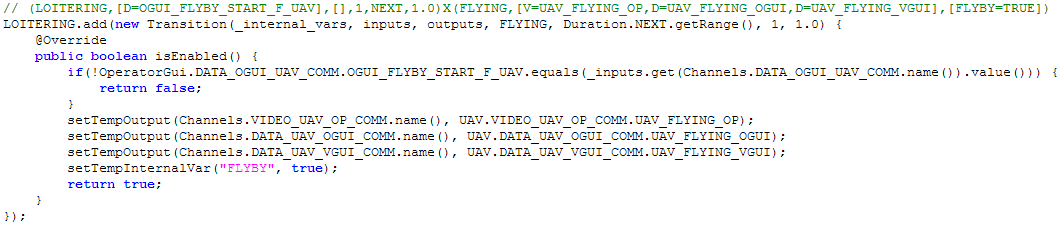
\includegraphics[width=\textwidth]{java_transition.png}
	\label{subfig:subtop}
}
\subfigure[XML Transition]{
	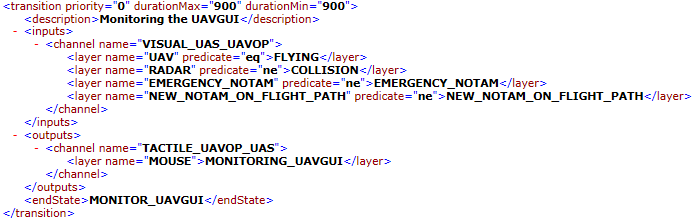
\includegraphics[width=\textwidth]{xml_transition.png}
	\label{subfig:subbot}
}
\caption{Transition Readability Comparison}
\label{fig:read_transition}
\end{center}
\end{figure}

The Enhanced Operator Function Model (EOFM), a similar modeling language which is XML based, is able to be seen visually as a tree-like graph due to the modeling structure~\cite{bolton2011toward}.  This visualization allows the modeler to see the hierarchical ordering of actions belonging to a task.  Our xml structure does not lend itself naturally to a visualization which grants additional insight into the model behavior.

\subsection{Modeling Approach and Common Errors}

Past experience has shown us that modeling these complex systems can become very difficult.  In an effort to reduce the complexity we used the following modeling approach.  We first defined each Actor in the system and gave them a starting state.  From here we broke the work into task sequences.  Each task sequence represents the flow of data through the system, initiating from an external event.  For example our model begins with a start mission event which is received by the UAV Operator.  We then implement transitions in sequence until no new transitions are needed.  Each time a new transition is added to the model we run the model to check that the XML is correct and to verify that the new transition is reached.  The full model can be seen in appendix~\ref{XMLModel}.

While this approach was effective it was not a trivial task.  By design the transition sequence moves between Actors requiring the modeler to constantly jump around in the model XML.  Transition sequences will often fork when the action of one Actor causes multiple Actors to respond.  This often results in truncated branches within the model which get forgotten.  One reason for running the model after adding a new transition is that when the complexity causes modeling errors they typically appear in two fashions.  The first is when an Actor becomes stuck in a state.  This is the more desirable behavior as it is easier to track down.  The second typical error is an infinite loop.  These can be much more difficult to track down.  Infinite loops are often caused by missing transitions, which is ok while constructing the model.  If the loop is not caused by a missing transition then more in-depth analysis is needed to find the error.  The Java debugger along with our different debug levels and outputs makes tracking down these errors rather straight forward although the process can be time consuming.  While there are many ways to get into an infinite loop we will only mention the two most common, they are improper transition overriding and uncleared output channels.  Transition overriding happens when you have one transition which is overridden by another before it can fire.  While transition overriding is a desirable behavior, gaps in the transition logic can cause an Actor to continuously cycle between transitions without ever firing a transition and moving to the next state. This can be thought of as undefined behavior.  To fix this, define the true behavior for each possible scenario by creating transitions for all combinations of inputs that the model cares about.  The simulator will prevent a transition from replacing itself preventing the infinite loop.  Uncleared output channels can cause an Actor to believe that a new value has been sent causing the Actor to transition into an infinite cycle.  It is often best practice to clear an Actors outputs once those outputs are no longer needed.

While the use of XML to create the model was much more efficient we still feel that a more effective approach to modeling is needed which helps standardize the modeling formats and prevent common errors.  Whether this approach is a different XML structure, an entirely new format, or a GUI interface which helps visualize the data flow and transition sequences we leave to future work.

\section{Model Results}

We were very impressed with the results generated with this new case study.  

\begin{figure}[p]
\begin{center}
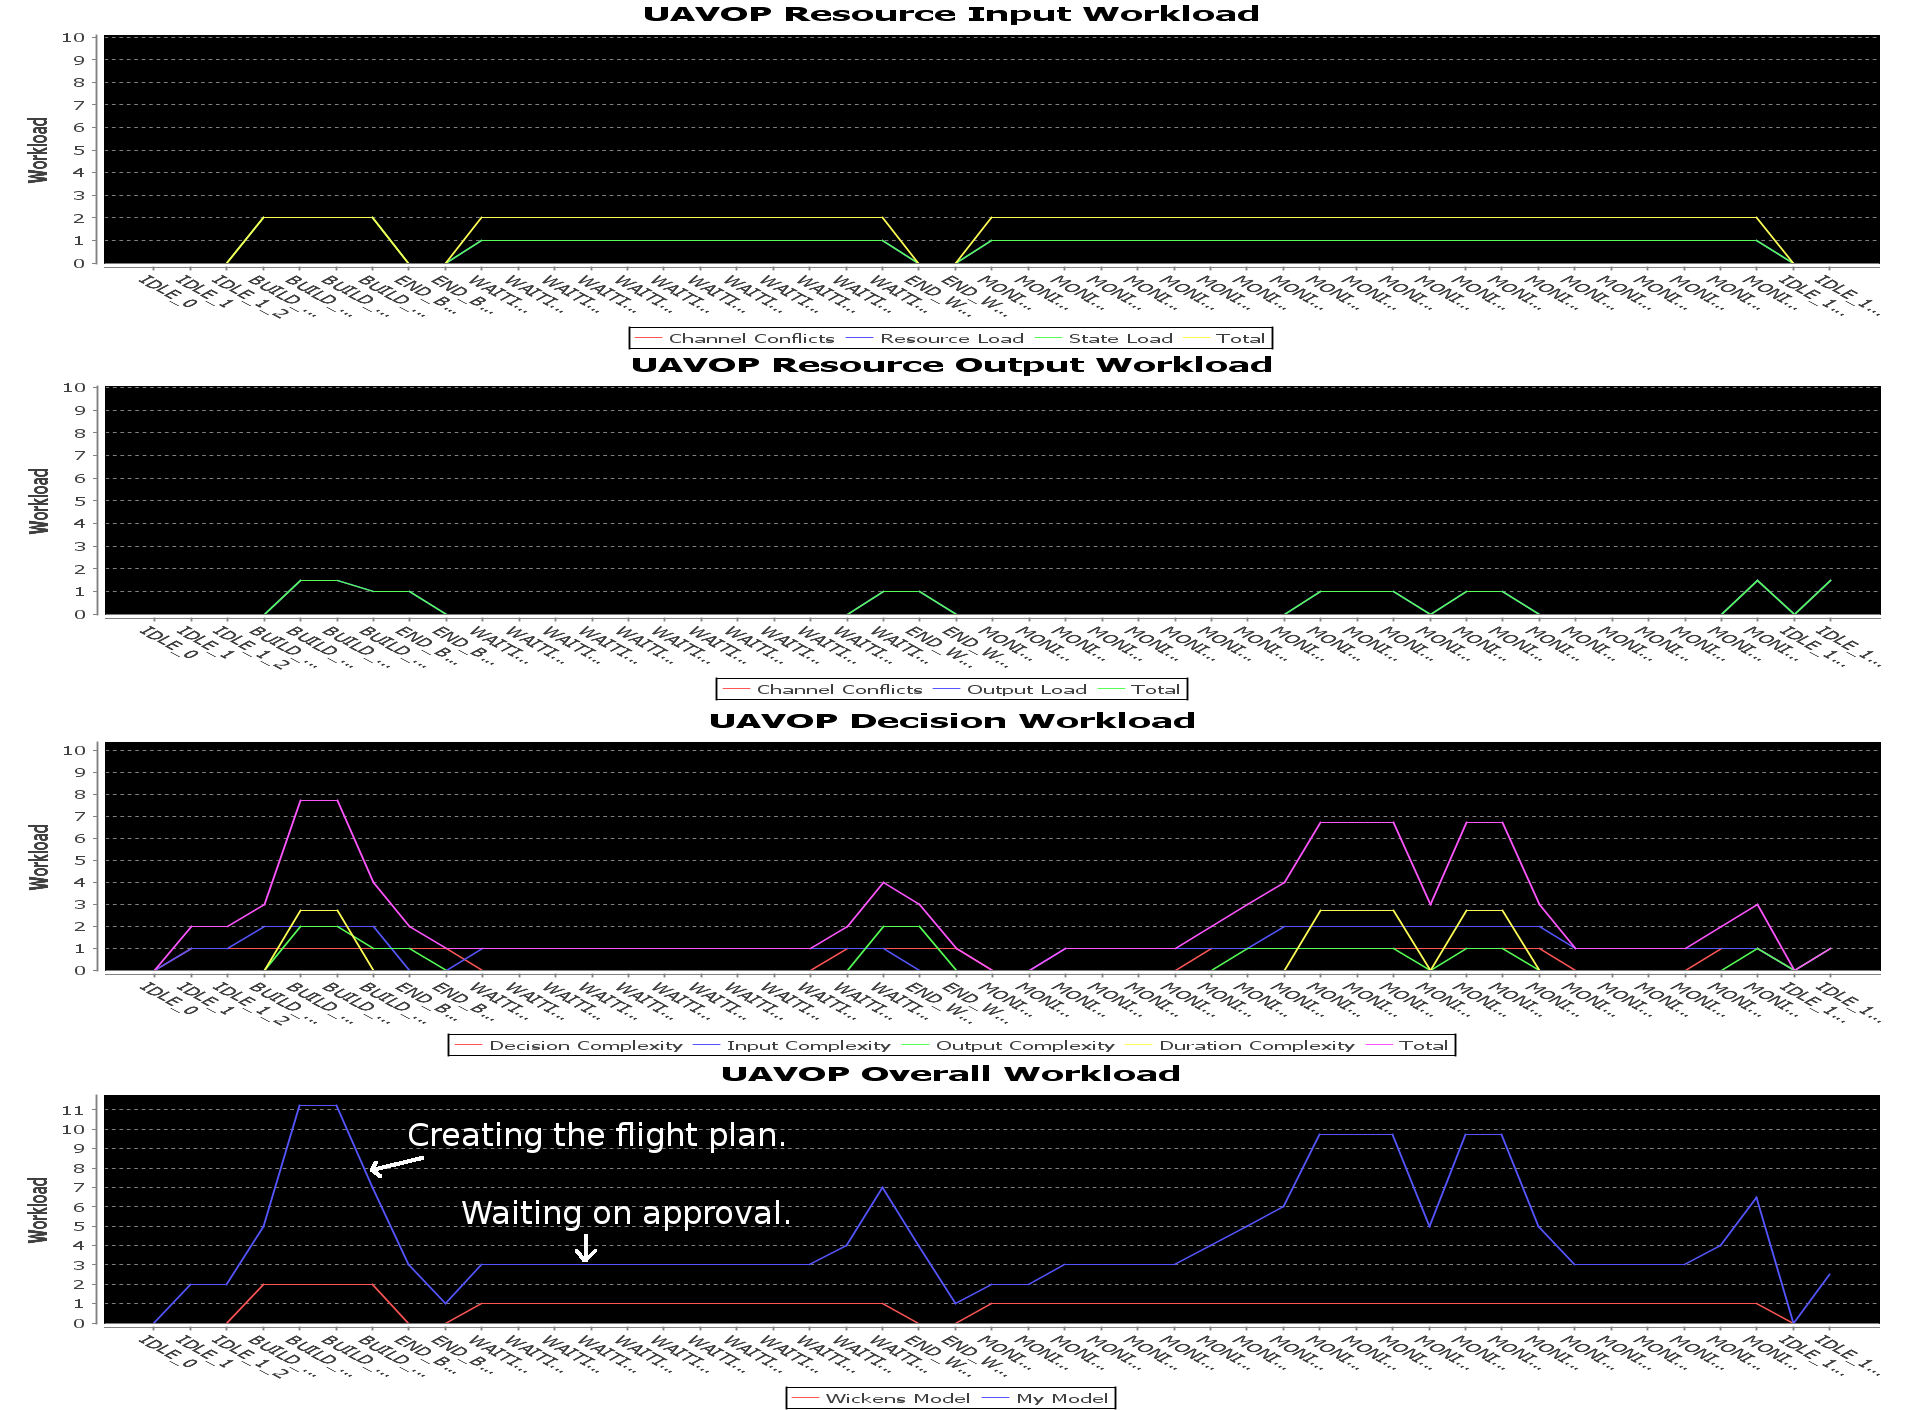
\includegraphics[width=\textwidth,height=\textheight]{UAS_in_NAS_no_events_UAVOP.png}
\caption{UAV Operator: Baseline}
\label{fig:uavop_baseline}
\end{center}
\end{figure}

\begin{figure}[p]
\begin{center}
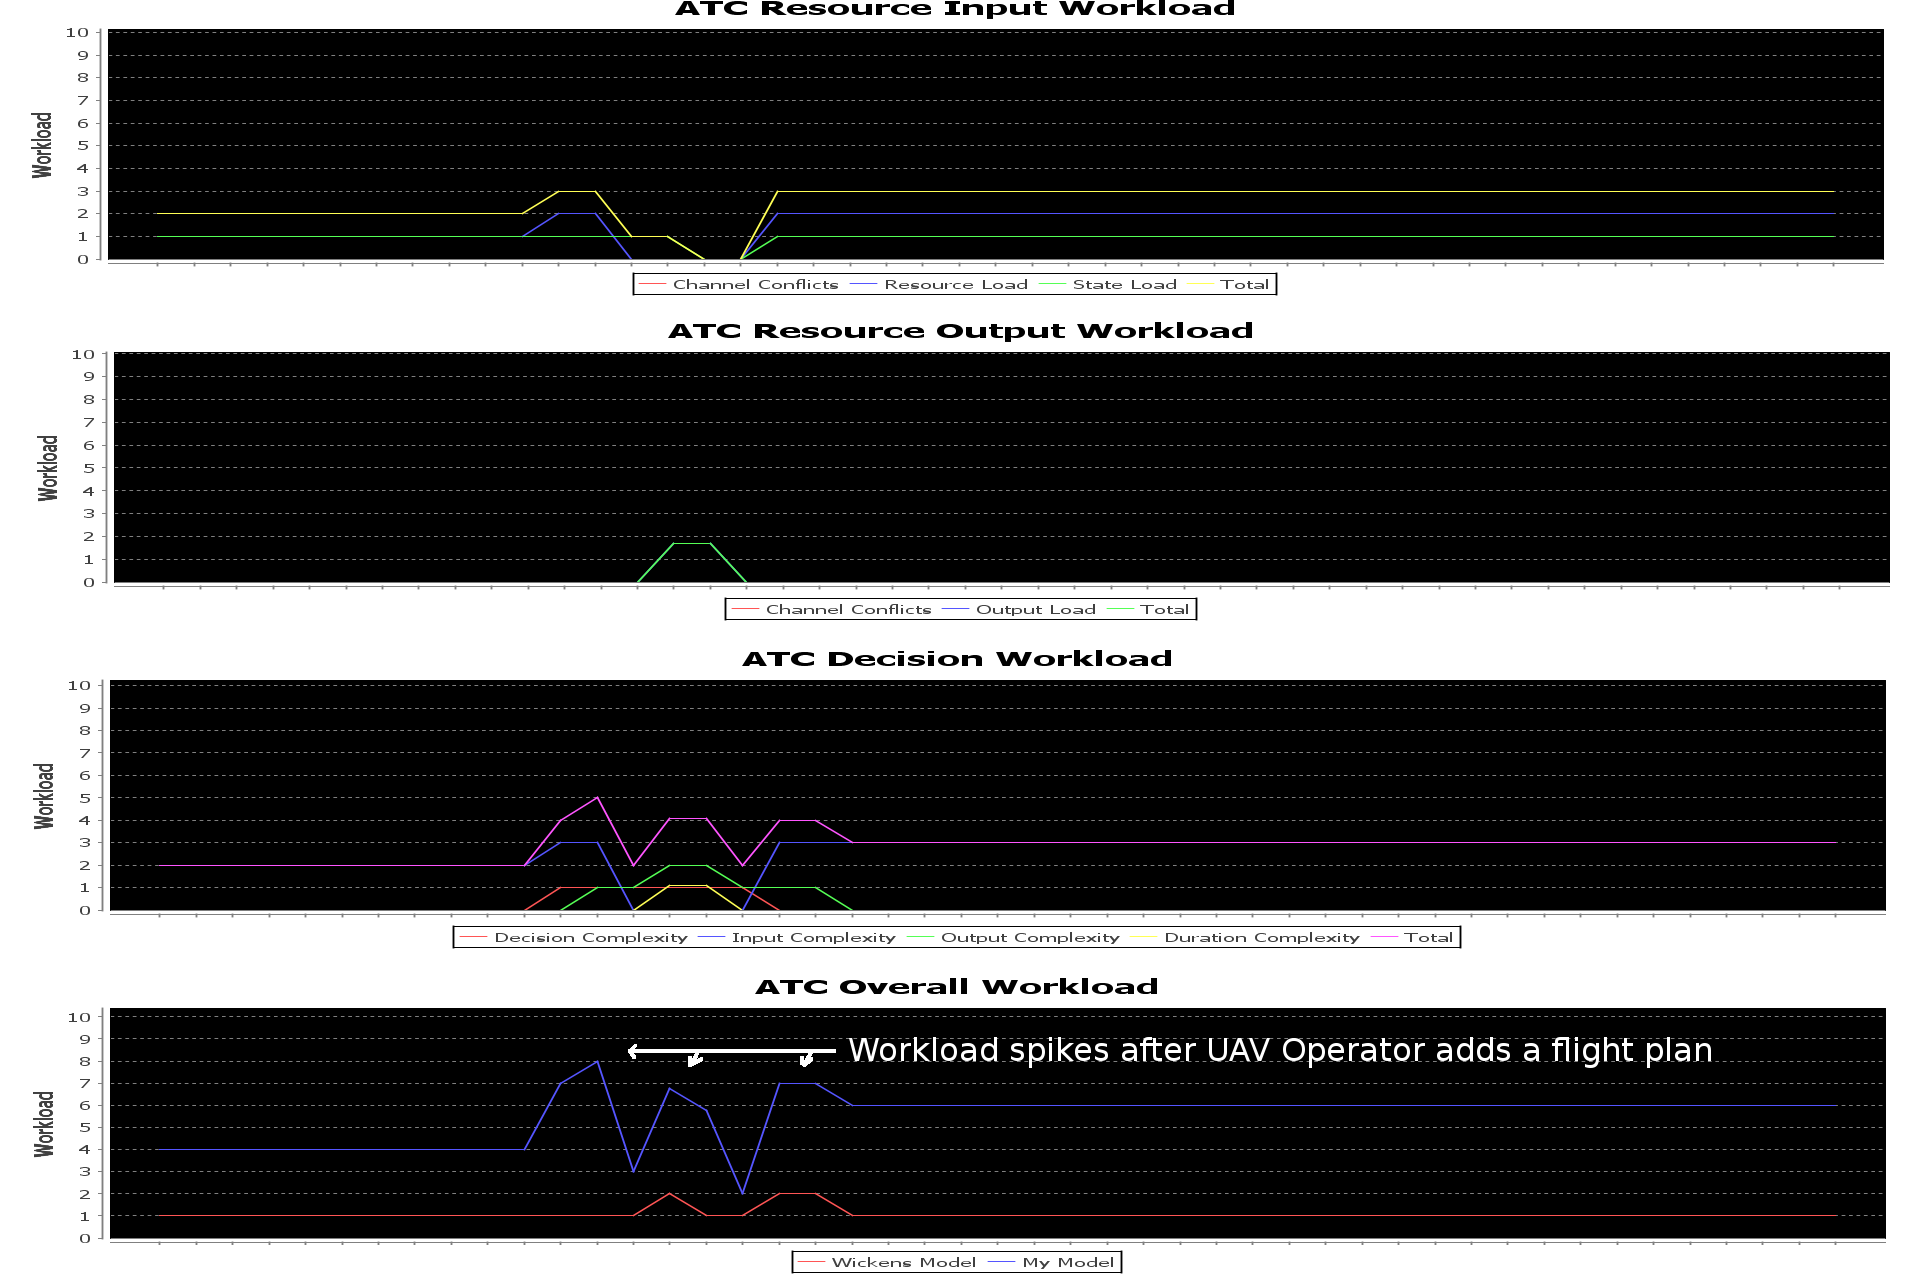
\includegraphics[width=\textwidth,height=\textheight]{UAS_in_NAS_no_events_ATC.png}
\caption{ATC: Baseline}
\label{fig:atc_baseline}
\end{center}
\end{figure}

\begin{figure}[p]
\begin{center}
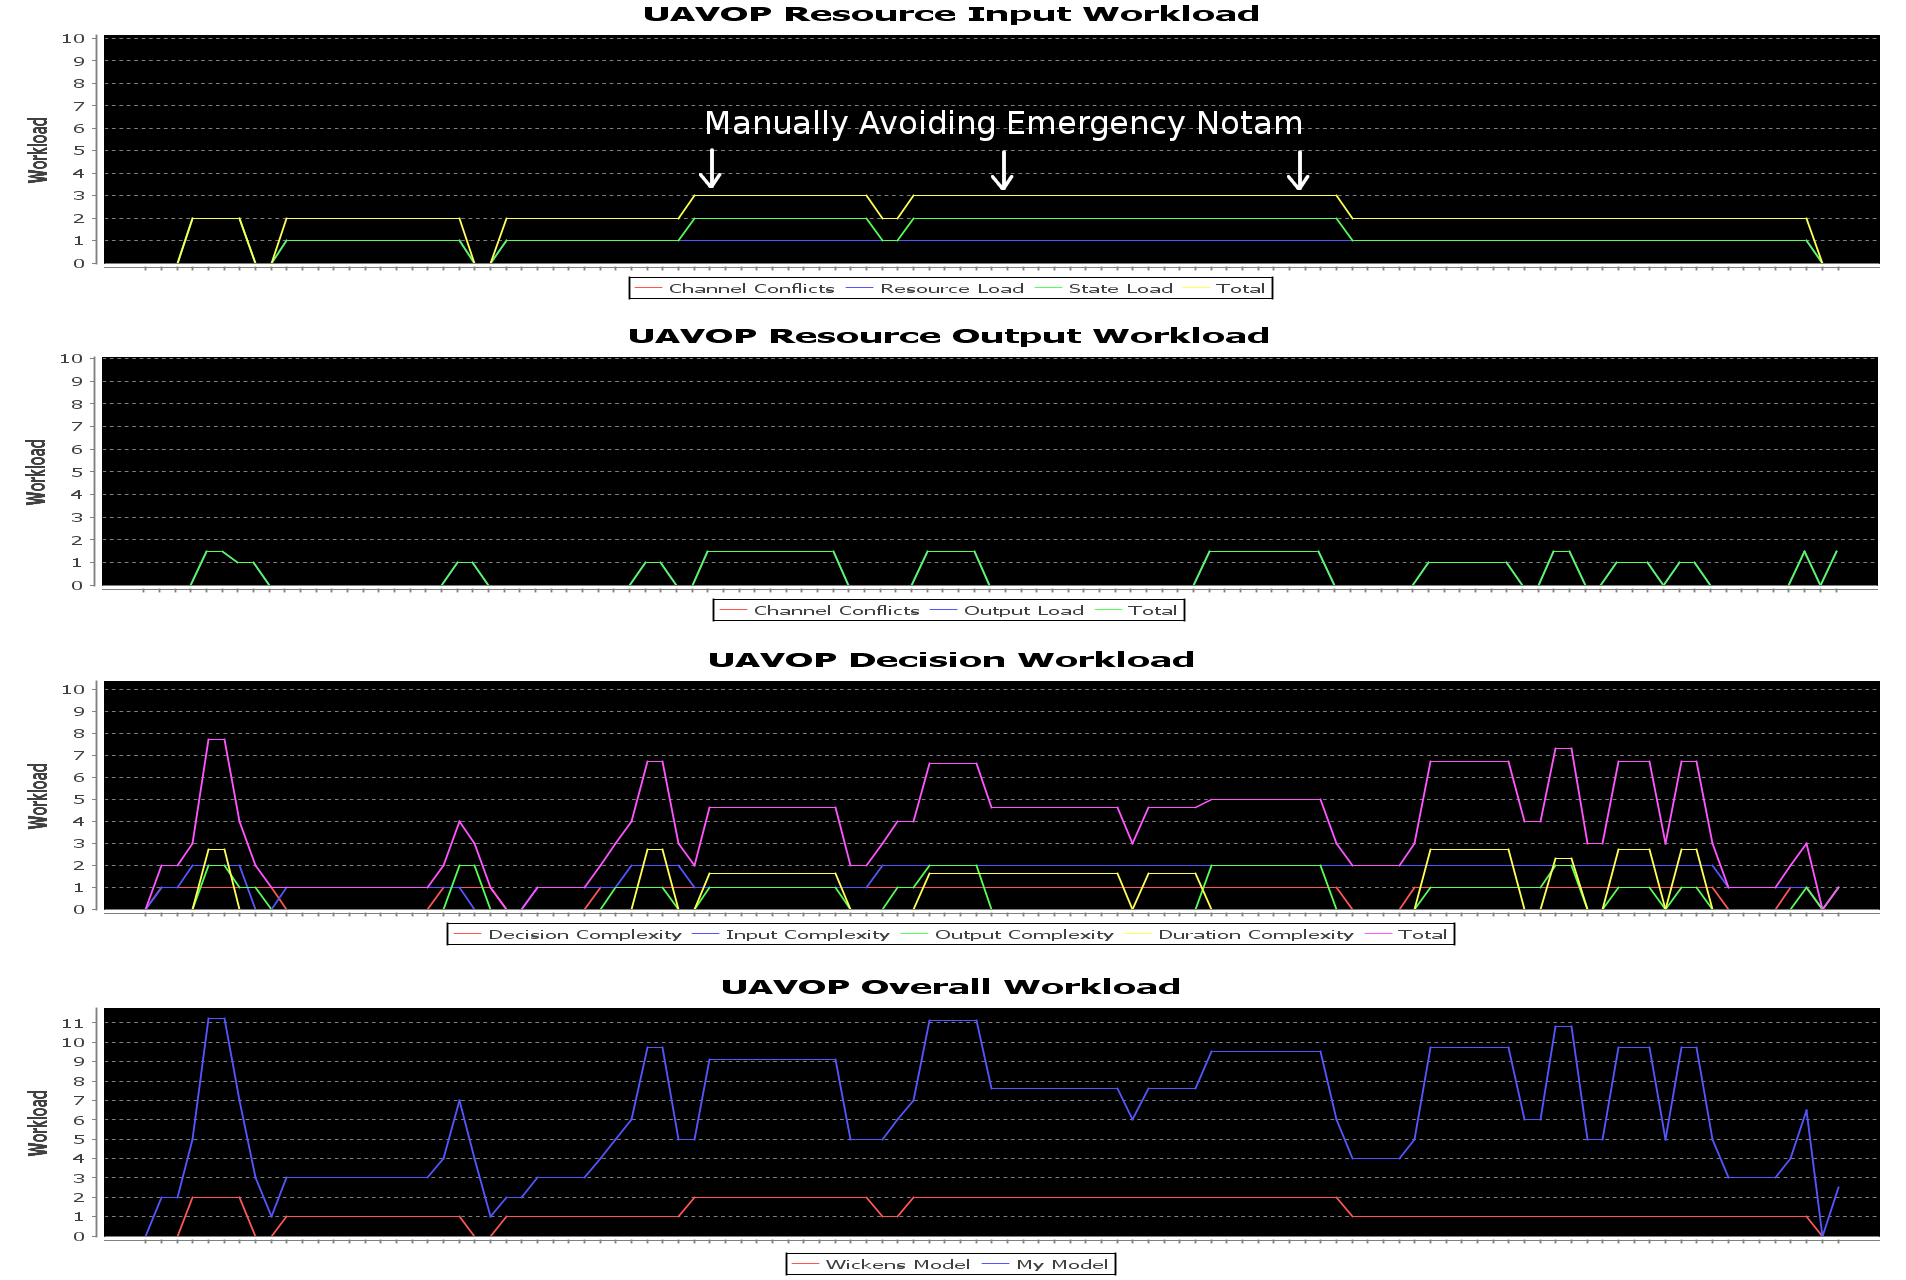
\includegraphics[width=\textwidth,height=\textheight]{UAS_in_NAS_manual_emergency_notam_UAVOP.png}
\caption{UAV Operator: Manually Avoided Emergency NOTAM}
\label{fig:uavop_manual}
\end{center}
\end{figure}

\begin{figure}[p]
\begin{center}
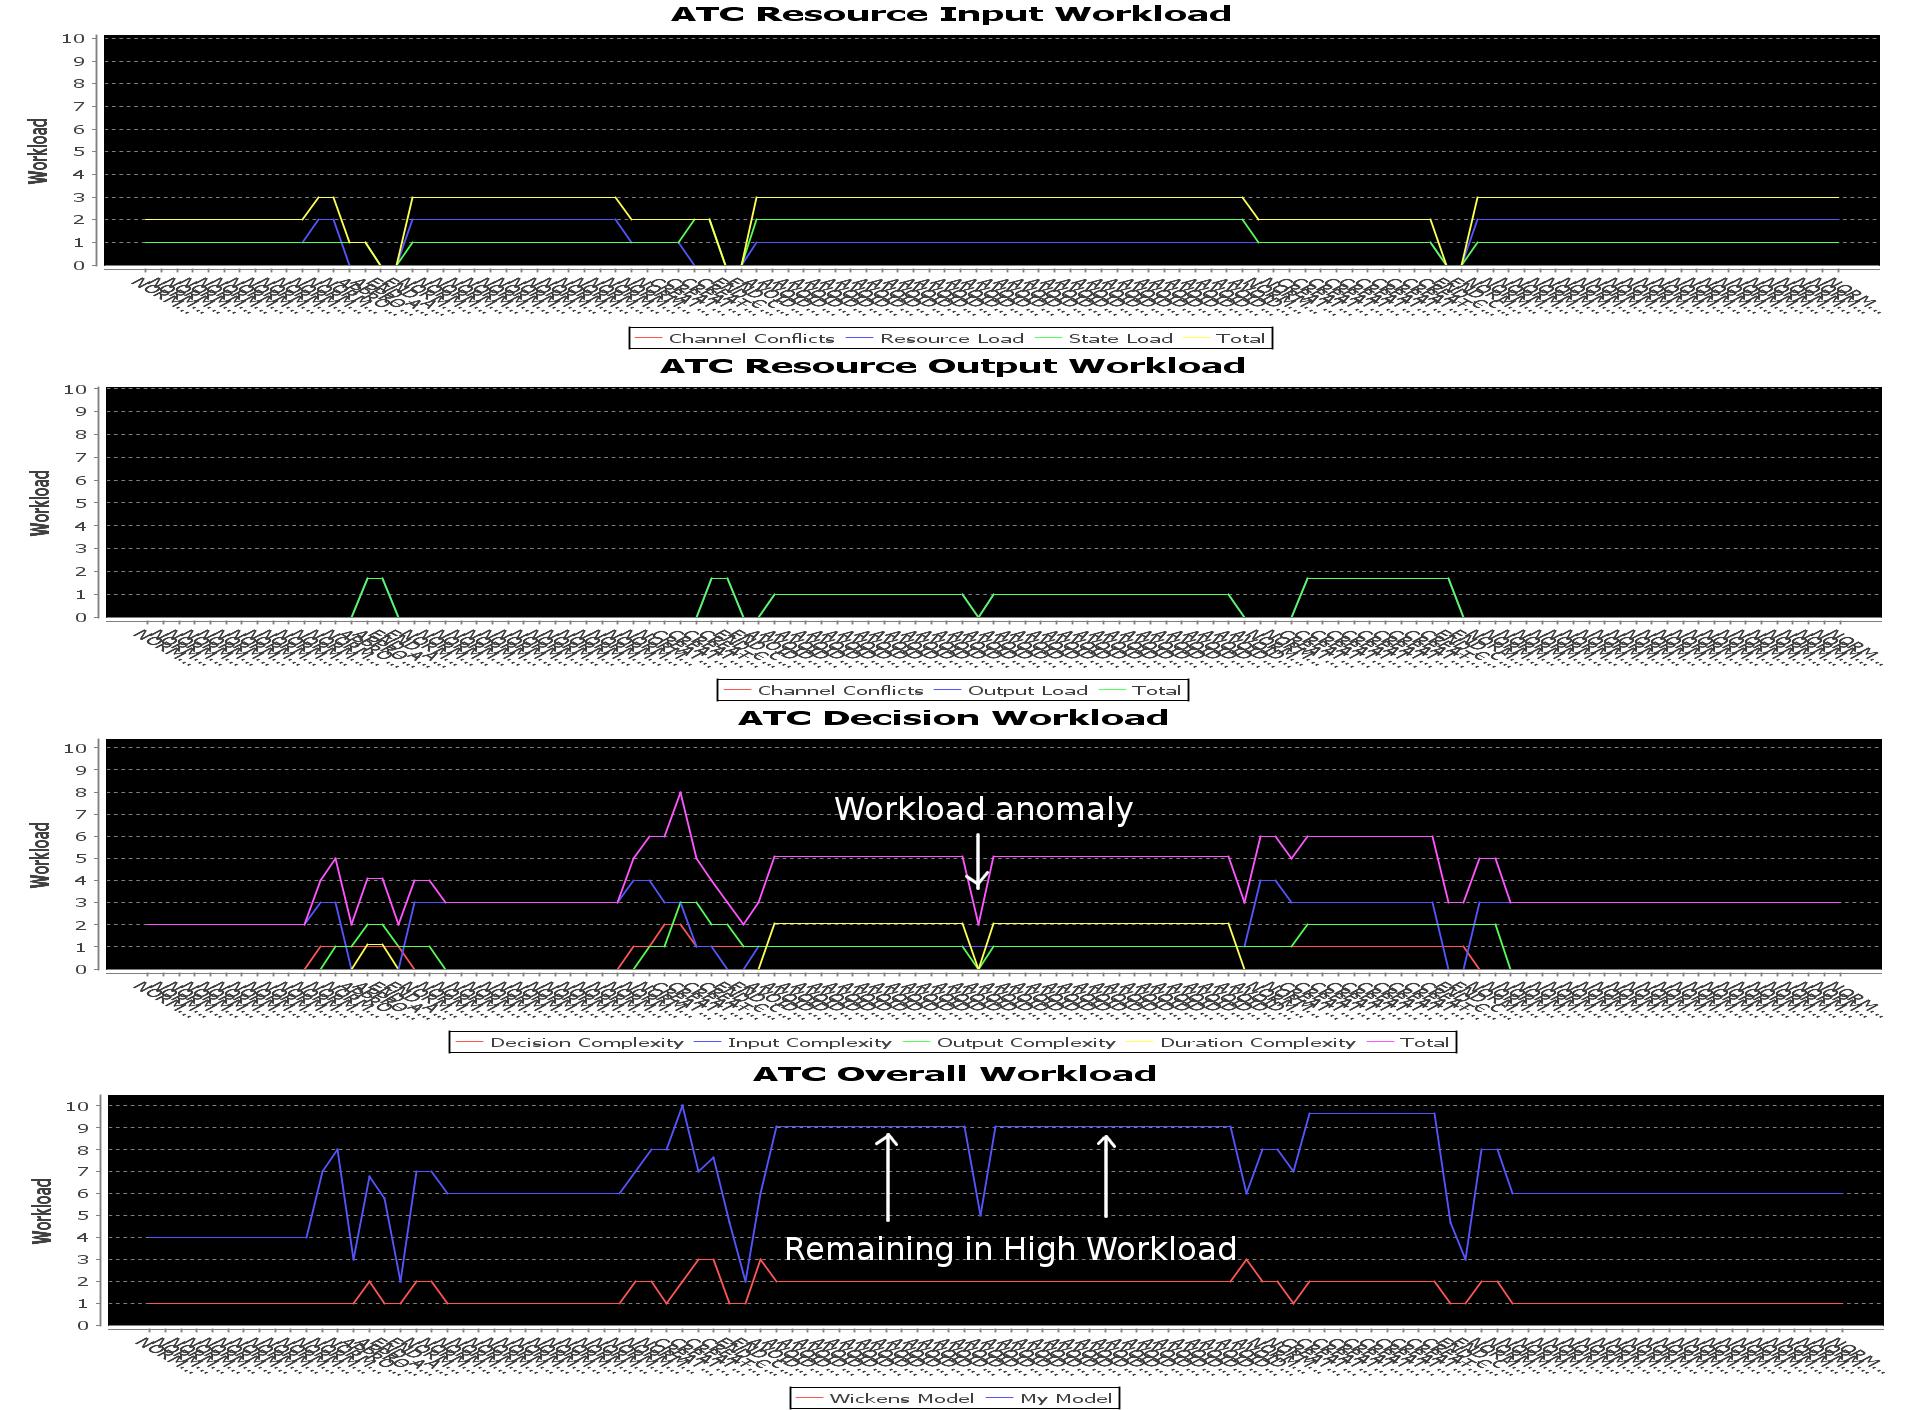
\includegraphics[width=\textwidth,height=\textheight]{UAS_in_NAS_manual_emergency_notam_ATC.png}
\caption{ATC: Manually Avoided Emergency NOTAM}
\label{fig:atc_manual}
\end{center}
\end{figure}

\begin{figure}[p]
\begin{center}
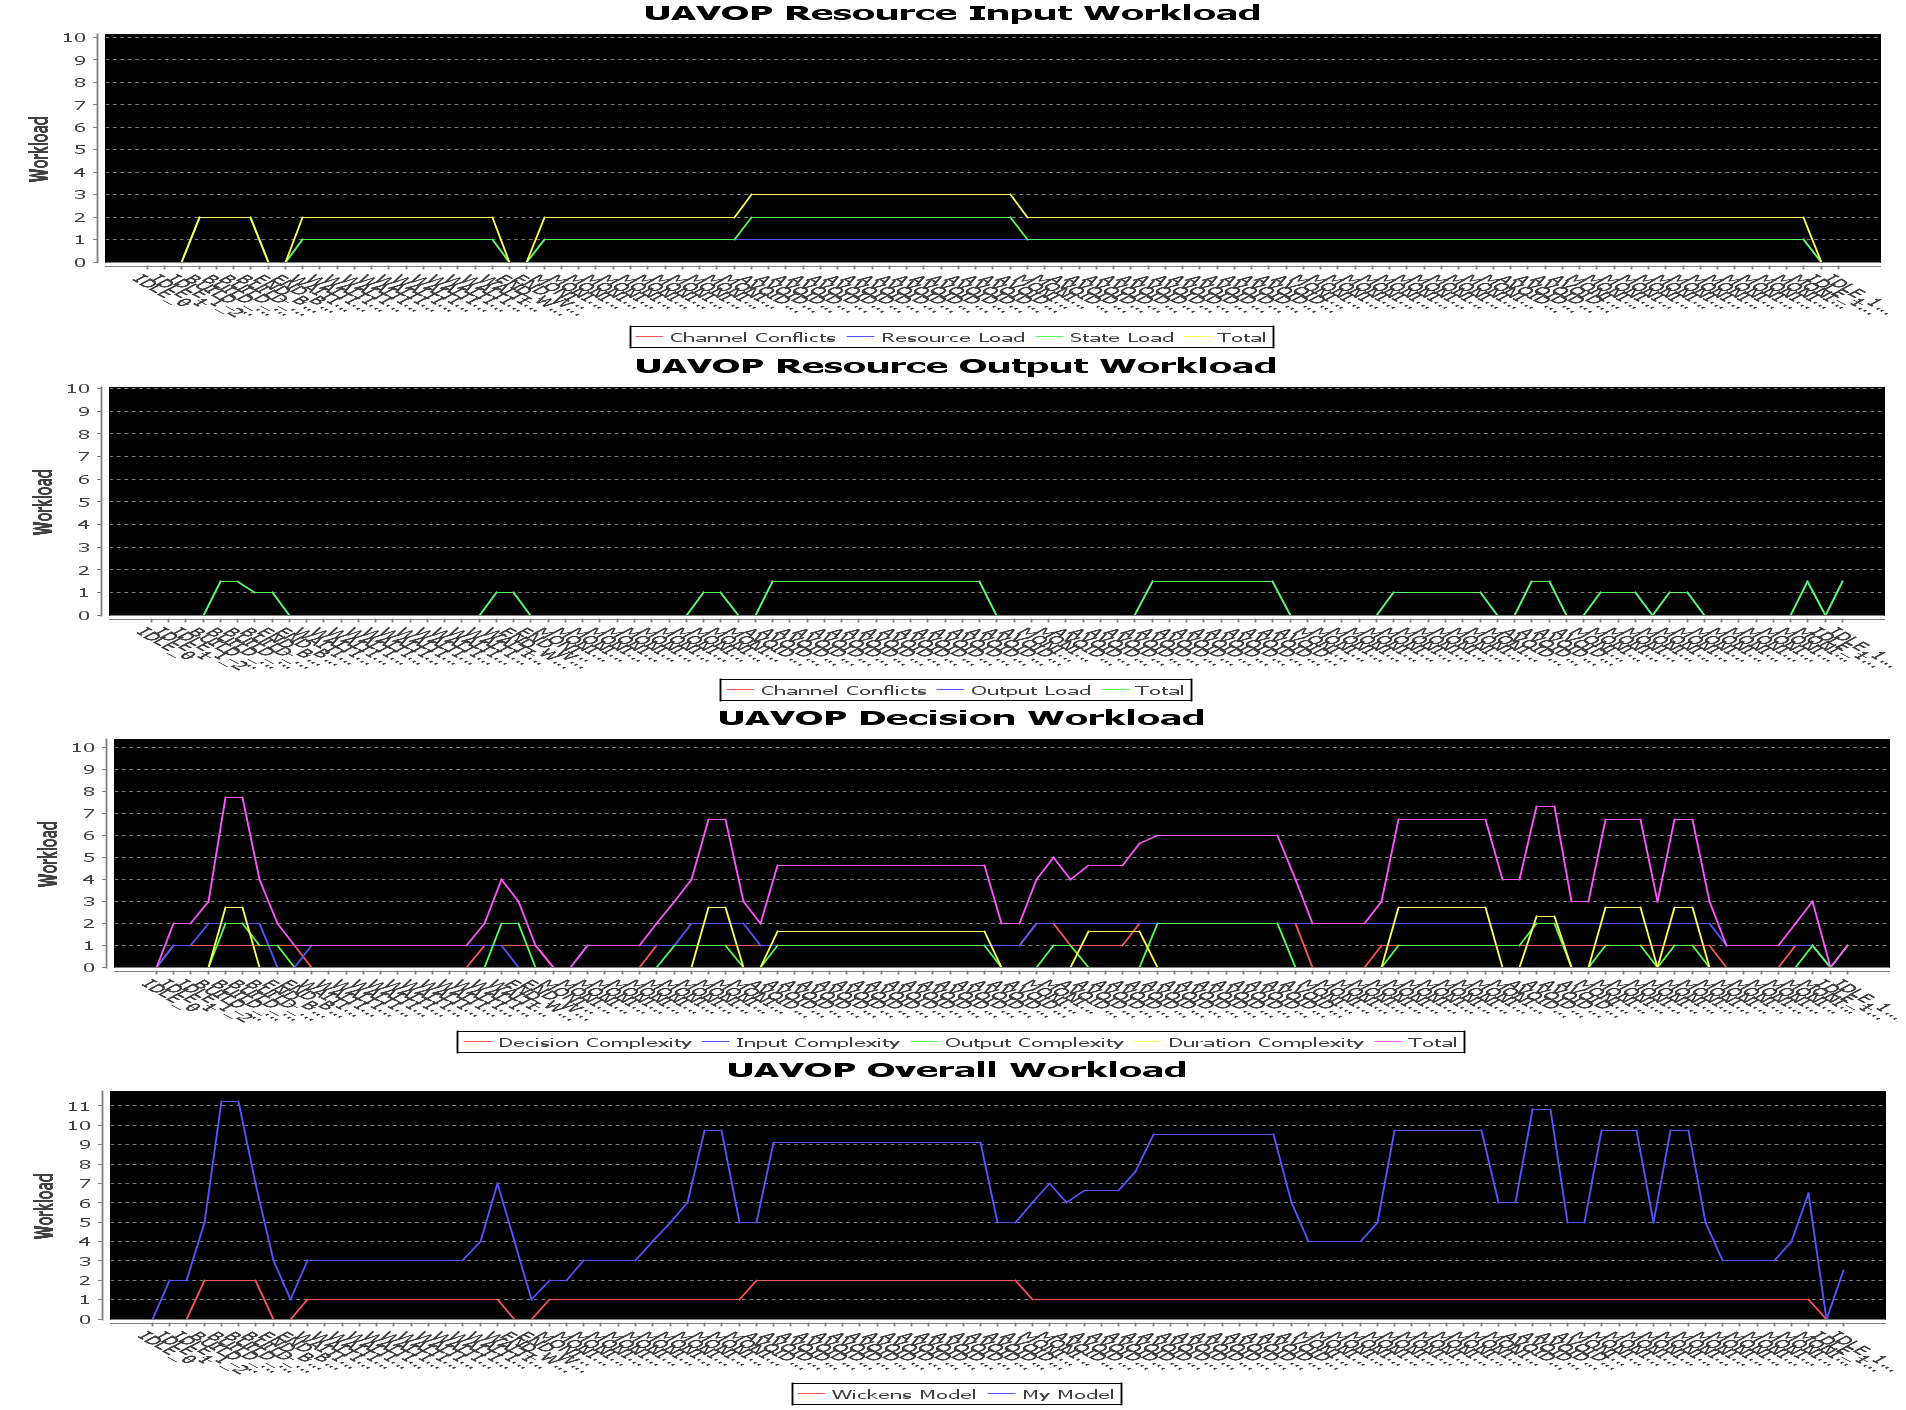
\includegraphics[width=\textwidth,height=\textheight]{UAS_in_NAS_auto_emergency_notam_UAVOP.png}
\caption{UAV Operator: Auto Avoid Emergency NOTAM}
\label{fig:uavop_auto}
\end{center}
\end{figure}

\begin{figure}[p]
\begin{center}
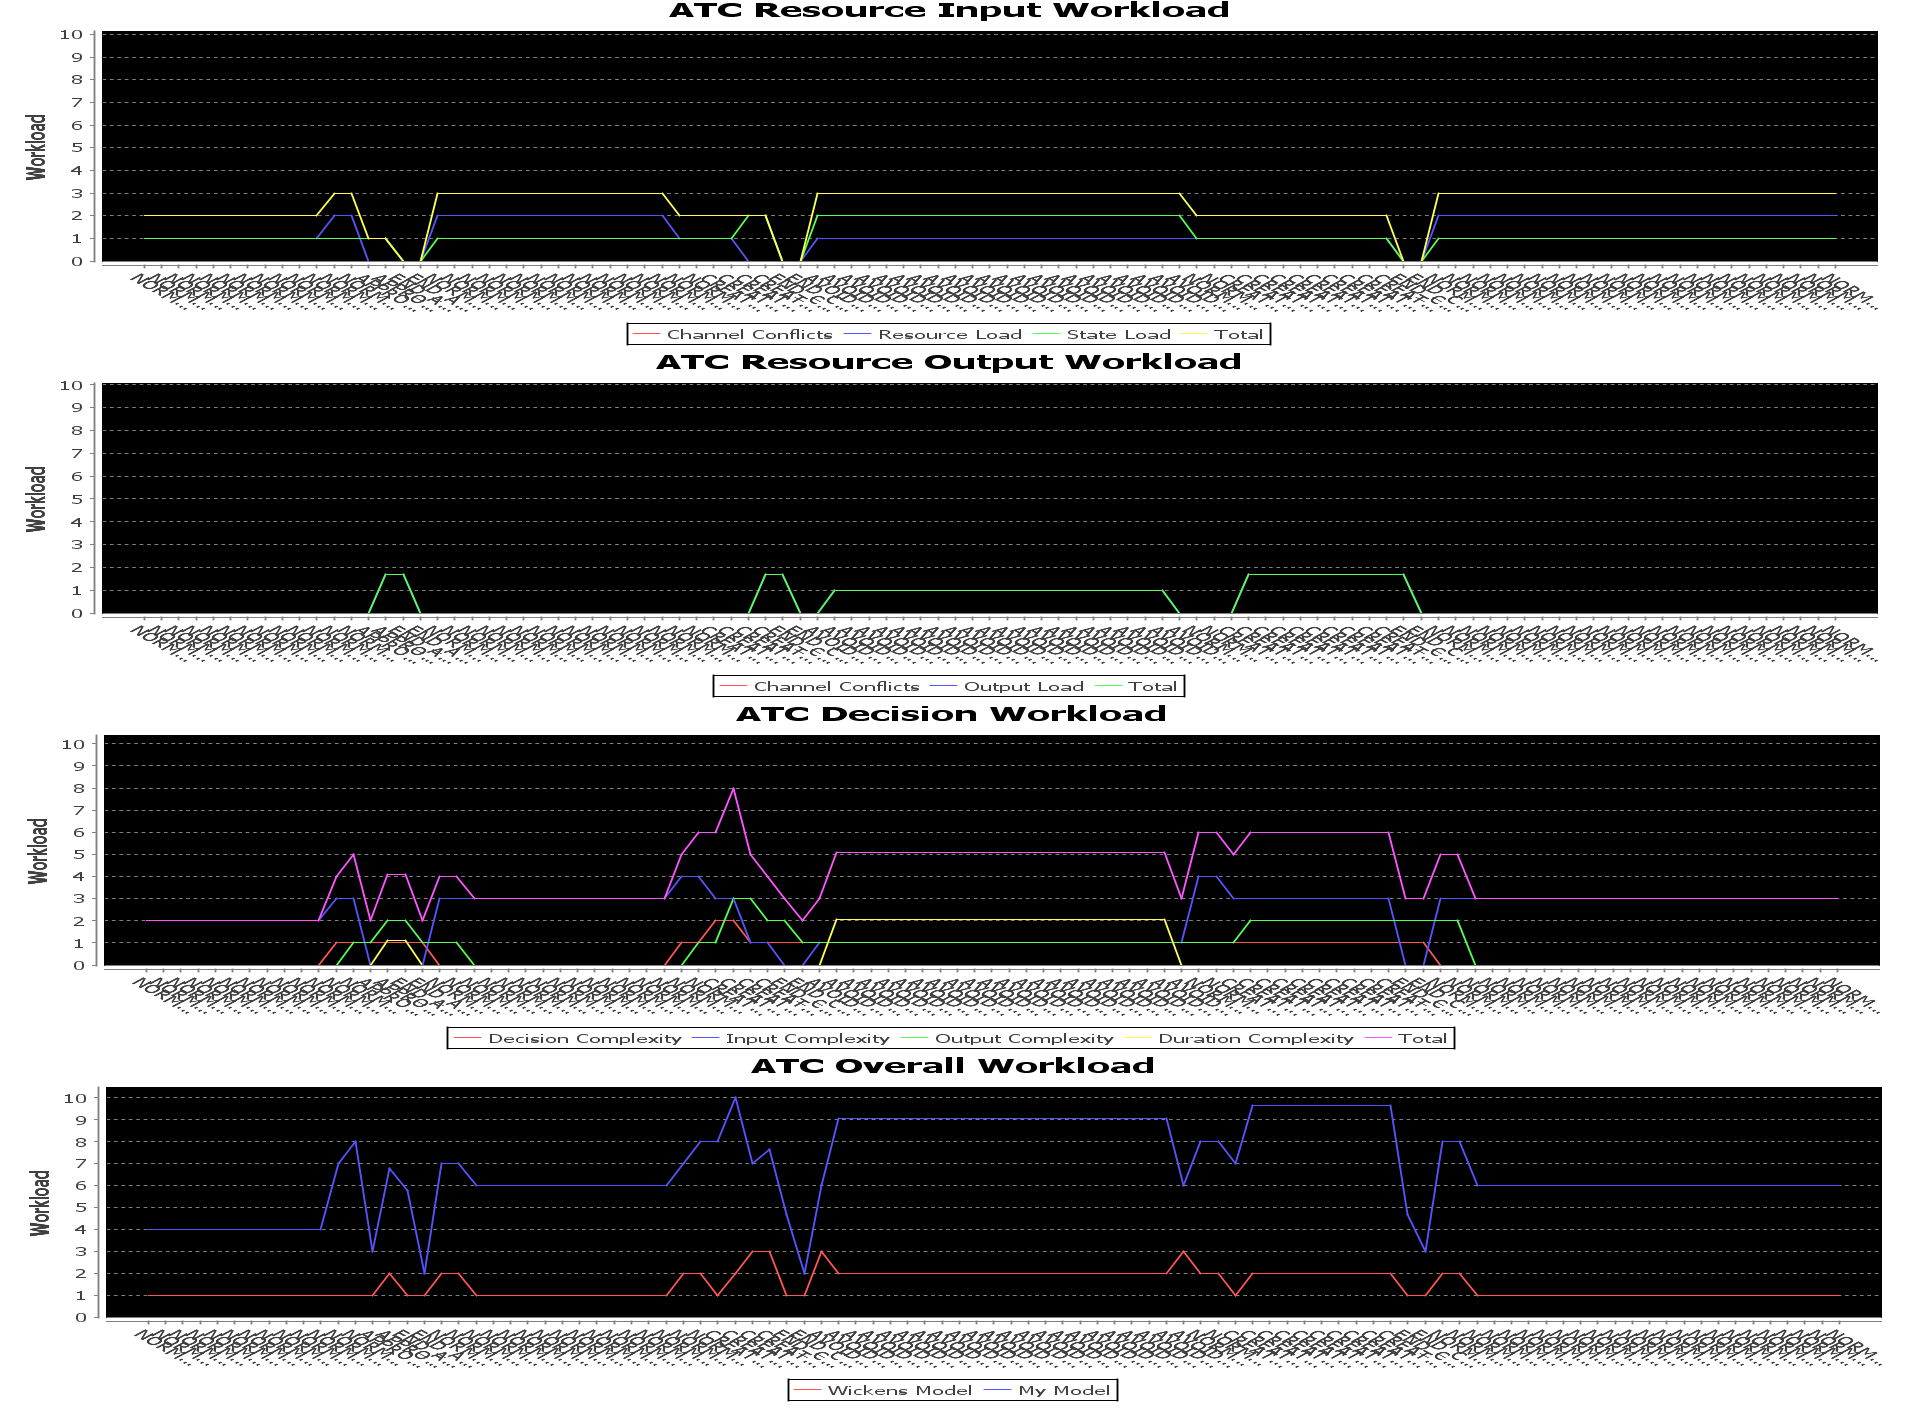
\includegraphics[width=\textwidth,height=\textheight]{UAS_in_NAS_auto_emergency_notam_ATC.png}
\caption{ATC: Auto Avoid Emergency NOTAM}
\label{fig:atc_auto}
\end{center}
\end{figure}
